\documentclass{extbook}[14pt]
\usepackage{multicol, enumerate, enumitem, hyperref, color, soul, setspace, parskip, fancyhdr, amssymb, amsthm, amsmath, latexsym, units, mathtools}
\everymath{\displaystyle}
\usepackage[headsep=0.5cm,headheight=0cm, left=1 in,right= 1 in,top= 1 in,bottom= 1 in]{geometry}
\usepackage{dashrule}  % Package to use the command below to create lines between items
\newcommand{\litem}[1]{\item #1

\rule{\textwidth}{0.4pt}}
\pagestyle{fancy}
\lhead{}
\chead{Answer Key for Progress Quiz 4 Version ALL}
\rhead{}
\lfoot{5346-5907}
\cfoot{}
\rfoot{Summer C 2021}
\begin{document}
\textbf{This key should allow you to understand why you choose the option you did (beyond just getting a question right or wrong). \href{https://xronos.clas.ufl.edu/mac1105spring2020/courseDescriptionAndMisc/Exams/LearningFromResults}{More instructions on how to use this key can be found here}.}

\textbf{If you have a suggestion to make the keys better, \href{https://forms.gle/CZkbZmPbC9XALEE88}{please fill out the short survey here}.}

\textit{Note: This key is auto-generated and may contain issues and/or errors. The keys are reviewed after each exam to ensure grading is done accurately. If there are issues (like duplicate options), they are noted in the offline gradebook. The keys are a work-in-progress to give students as many resources to improve as possible.}

\rule{\textwidth}{0.4pt}

\begin{enumerate}\litem{
Construct the lowest-degree polynomial given the zeros below. Then, choose the intervals that contain the coefficients of the polynomial in the form $ax^3+bx^2+cx+d$.
\[ \frac{2}{3}, -7, \text{ and } \frac{7}{5} \]The solution is \( 15x^{3} +74 x^{2} -203 x + 98 \), which is option A.\begin{enumerate}[label=\Alph*.]
\item \( a \in [14, 16], b \in [74, 75], c \in [-204, -195], \text{ and } d \in [97, 102] \)

* $15x^{3} +74 x^{2} -203 x + 98$, which is the correct option.
\item \( a \in [14, 16], b \in [74, 75], c \in [-204, -195], \text{ and } d \in [-98, -96] \)

$15x^{3} +74 x^{2} -203 x -98$, which corresponds to multiplying everything correctly except the constant term.
\item \( a \in [14, 16], b \in [83, 101], c \in [-98, -83], \text{ and } d \in [-98, -96] \)

$15x^{3} +94 x^{2} -91 x -98$, which corresponds to multiplying out $(3x + 2)(x + 7)(5x -7)$.
\item \( a \in [14, 16], b \in [-81, -66], c \in [-204, -195], \text{ and } d \in [-98, -96] \)

$15x^{3} -74 x^{2} -203 x -98$, which corresponds to multiplying out $(3x + 2)(x -7)(5x + 7)$.
\item \( a \in [14, 16], b \in [-116, -113], c \in [62, 71], \text{ and } d \in [97, 102] \)

$15x^{3} -116 x^{2} +63 x + 98$, which corresponds to multiplying out $(3x + 2)(x -7)(5x -7)$.
\end{enumerate}

\textbf{General Comment:} To construct the lowest-degree polynomial, you want to multiply out $(3x -2)(x + 7)(5x -7)$
}
\litem{
Describe the zero behavior of the zero $x = 8$ of the polynomial below.
\[ f(x) = -4(x + 8)^{7}(x - 8)^{10}(x - 4)^{4}(x + 4)^{8} \]The solution is the graph below, which is option B.
    \begin{center}
        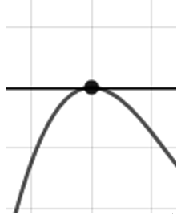
\includegraphics[width=0.3\textwidth]{../Figures/polyZeroBehaviorBA.png}
    \end{center}\begin{enumerate}[label=\Alph*.]
\begin{multicols}{2}
\item 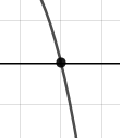
\includegraphics[width = 0.3\textwidth]{../Figures/polyZeroBehaviorAA.png}
\item 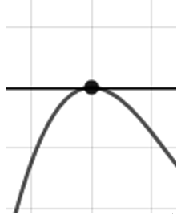
\includegraphics[width = 0.3\textwidth]{../Figures/polyZeroBehaviorBA.png}
\item 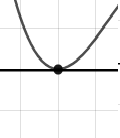
\includegraphics[width = 0.3\textwidth]{../Figures/polyZeroBehaviorCA.png}
\item 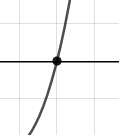
\includegraphics[width = 0.3\textwidth]{../Figures/polyZeroBehaviorDA.png}
\end{multicols}\item None of the above.\end{enumerate}
\textbf{General Comment:} You will need to sketch the entire graph, then zoom in on the zero the question asks about.
}
\litem{
Construct the lowest-degree polynomial given the zeros below. Then, choose the intervals that contain the coefficients of the polynomial in the form $x^3+bx^2+cx+d$.
\[ -2 + 4 i \text{ and } 4 \]The solution is \( x^{3} +4 x -80 \), which is option D.\begin{enumerate}[label=\Alph*.]
\item \( b \in [0.9, 2.6], c \in [-10, -4.4], \text{ and } d \in [15, 18] \)

$x^{3} + x^{2} -8 x + 16$, which corresponds to multiplying out $(x -4)(x -4)$.
\item \( b \in [-3.1, 0.1], c \in [2.6, 4.7], \text{ and } d \in [79, 82] \)

$x^{3} +4 x + 80$, which corresponds to multiplying out $(x-(-2 + 4 i))(x-(-2 - 4 i))(x + 4)$.
\item \( b \in [0.9, 2.6], c \in [-6.7, 0.2], \text{ and } d \in [-12, -6] \)

$x^{3} + x^{2} -2 x -8$, which corresponds to multiplying out $(x + 2)(x -4)$.
\item \( b \in [-3.1, 0.1], c \in [2.6, 4.7], \text{ and } d \in [-82, -75] \)

* $x^{3} +4 x -80$, which is the correct option.
\item \( \text{None of the above.} \)

This corresponds to making an unanticipated error or not understanding how to use nonreal complex numbers to create the lowest-degree polynomial. If you chose this and are not sure what you did wrong, please contact the coordinator for help.
\end{enumerate}

\textbf{General Comment:} Remember that the conjugate of $a+bi$ is $a-bi$. Since these zeros always come in pairs, we need to multiply out $(x-(-2 + 4 i))(x-(-2 - 4 i))(x-(4))$.
}
\litem{
Which of the following equations \textit{could} be of the graph presented below?

\begin{center}
    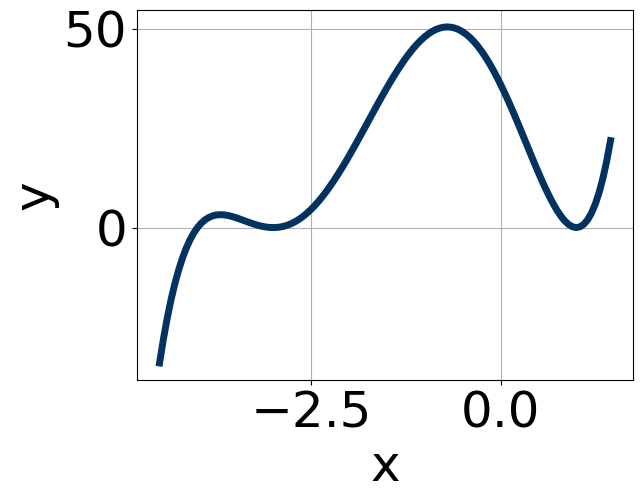
\includegraphics[width=0.5\textwidth]{../Figures/polyGraphToFunctionCopyA.png}
\end{center}


The solution is \( 15(x - 1)^{4} (x + 3)^{8} (x + 4)^{5} \), which is option B.\begin{enumerate}[label=\Alph*.]
\item \( 3(x - 1)^{8} (x + 3)^{7} (x + 4)^{9} \)

The factor $(x + 3)$ should have an even power.
\item \( 15(x - 1)^{4} (x + 3)^{8} (x + 4)^{5} \)

* This is the correct option.
\item \( 13(x - 1)^{10} (x + 3)^{7} (x + 4)^{6} \)

The factor $(x + 3)$ should have an even power and the factor $(x + 4)$ should have an odd power.
\item \( -5(x - 1)^{6} (x + 3)^{4} (x + 4)^{4} \)

The factor $(x + 4)$ should have an odd power and the leading coefficient should be the opposite sign.
\item \( -11(x - 1)^{10} (x + 3)^{10} (x + 4)^{7} \)

This corresponds to the leading coefficient being the opposite value than it should be.
\end{enumerate}

\textbf{General Comment:} General Comments: Draw the x-axis to determine which zeros are touching (and so have even multiplicity) or cross (and have odd multiplicity).
}
\litem{
Describe the zero behavior of the zero $x = -5$ of the polynomial below.
\[ f(x) = 6(x + 8)^{4}(x - 8)^{2}(x - 5)^{5}(x + 5)^{2} \]The solution is the graph below, which is option B.
    \begin{center}
        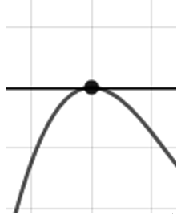
\includegraphics[width=0.3\textwidth]{../Figures/polyZeroBehaviorCopyBA.png}
    \end{center}\begin{enumerate}[label=\Alph*.]
\begin{multicols}{2}
\item 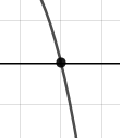
\includegraphics[width = 0.3\textwidth]{../Figures/polyZeroBehaviorCopyAA.png}
\item 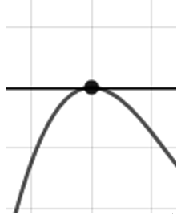
\includegraphics[width = 0.3\textwidth]{../Figures/polyZeroBehaviorCopyBA.png}
\item 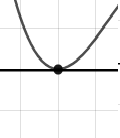
\includegraphics[width = 0.3\textwidth]{../Figures/polyZeroBehaviorCopyCA.png}
\item 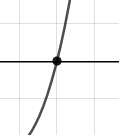
\includegraphics[width = 0.3\textwidth]{../Figures/polyZeroBehaviorCopyDA.png}
\end{multicols}\item None of the above.\end{enumerate}
\textbf{General Comment:} You will need to sketch the entire graph, then zoom in on the zero the question asks about.
}
\litem{
Which of the following equations \textit{could} be of the graph presented below?

\begin{center}
    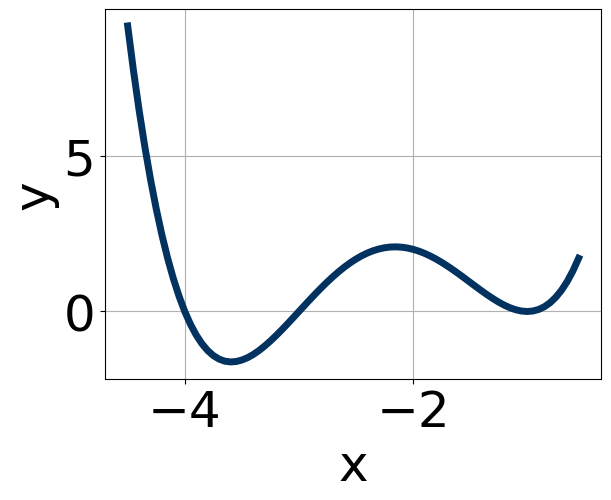
\includegraphics[width=0.5\textwidth]{../Figures/polyGraphToFunctionA.png}
\end{center}


The solution is \( 7(x + 1)^{8} (x + 3)^{9} (x + 4)^{11} \), which is option C.\begin{enumerate}[label=\Alph*.]
\item \( -7(x + 1)^{6} (x + 3)^{9} (x + 4)^{7} \)

This corresponds to the leading coefficient being the opposite value than it should be.
\item \( 3(x + 1)^{5} (x + 3)^{4} (x + 4)^{5} \)

The factor $-1$ should have an even power and the factor $-3$ should have an odd power.
\item \( 7(x + 1)^{8} (x + 3)^{9} (x + 4)^{11} \)

* This is the correct option.
\item \( -7(x + 1)^{4} (x + 3)^{9} (x + 4)^{10} \)

The factor $(x + 4)$ should have an odd power and the leading coefficient should be the opposite sign.
\item \( 17(x + 1)^{6} (x + 3)^{8} (x + 4)^{5} \)

The factor $(x + 3)$ should have an odd power.
\end{enumerate}

\textbf{General Comment:} General Comments: Draw the x-axis to determine which zeros are touching (and so have even multiplicity) or cross (and have odd multiplicity).
}
\litem{
Construct the lowest-degree polynomial given the zeros below. Then, choose the intervals that contain the coefficients of the polynomial in the form $x^3+bx^2+cx+d$.
\[ 5 + 4 i \text{ and } 2 \]The solution is \( x^{3} -12 x^{2} +61 x -82 \), which is option A.\begin{enumerate}[label=\Alph*.]
\item \( b \in [-20, -7], c \in [60, 64.2], \text{ and } d \in [-82.1, -78.6] \)

* $x^{3} -12 x^{2} +61 x -82$, which is the correct option.
\item \( b \in [-4, 6], c \in [-9.6, -6.6], \text{ and } d \in [8.9, 14] \)

$x^{3} + x^{2} -7 x + 10$, which corresponds to multiplying out $(x -5)(x -2)$.
\item \( b \in [12, 16], c \in [60, 64.2], \text{ and } d \in [79, 82.4] \)

$x^{3} +12 x^{2} +61 x + 82$, which corresponds to multiplying out $(x-(5 + 4 i))(x-(5 - 4 i))(x + 2)$.
\item \( b \in [-4, 6], c \in [-6.7, -2.2], \text{ and } d \in [4.9, 9.8] \)

$x^{3} + x^{2} -6 x + 8$, which corresponds to multiplying out $(x -4)(x -2)$.
\item \( \text{None of the above.} \)

This corresponds to making an unanticipated error or not understanding how to use nonreal complex numbers to create the lowest-degree polynomial. If you chose this and are not sure what you did wrong, please contact the coordinator for help.
\end{enumerate}

\textbf{General Comment:} Remember that the conjugate of $a+bi$ is $a-bi$. Since these zeros always come in pairs, we need to multiply out $(x-(5 + 4 i))(x-(5 - 4 i))(x-(2))$.
}
\litem{
Describe the end behavior of the polynomial below.
\[ f(x) = 7(x + 8)^{4}(x - 8)^{7}(x + 3)^{3}(x - 3)^{3} \]The solution is the graph below, which is option D.
    \begin{center}
        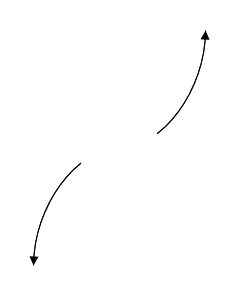
\includegraphics[width=0.3\textwidth]{../Figures/polyEndBehaviorCopyDA.png}
    \end{center}\begin{enumerate}[label=\Alph*.]
\begin{multicols}{2}
\item 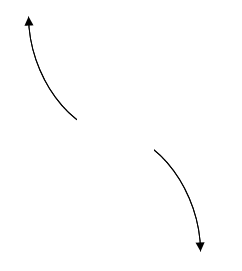
\includegraphics[width = 0.3\textwidth]{../Figures/polyEndBehaviorCopyAA.png}
\item 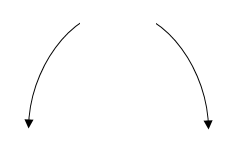
\includegraphics[width = 0.3\textwidth]{../Figures/polyEndBehaviorCopyBA.png}
\item 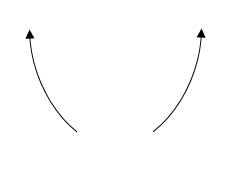
\includegraphics[width = 0.3\textwidth]{../Figures/polyEndBehaviorCopyCA.png}
\item 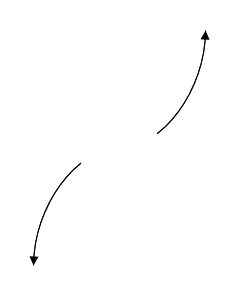
\includegraphics[width = 0.3\textwidth]{../Figures/polyEndBehaviorCopyDA.png}
\end{multicols}\item None of the above.\end{enumerate}
\textbf{General Comment:} Remember that end behavior is determined by the leading coefficient AND whether the \textbf{sum} of the multiplicities is positive or negative.
}
\litem{
Describe the end behavior of the polynomial below.
\[ f(x) = 5(x + 5)^{3}(x - 5)^{8}(x - 7)^{3}(x + 7)^{3} \]The solution is the graph below, which is option D.
    \begin{center}
        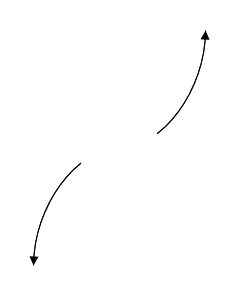
\includegraphics[width=0.3\textwidth]{../Figures/polyEndBehaviorDA.png}
    \end{center}\begin{enumerate}[label=\Alph*.]
\begin{multicols}{2}
\item 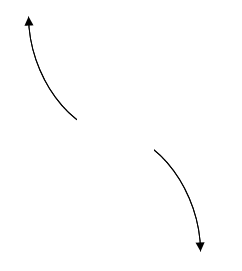
\includegraphics[width = 0.3\textwidth]{../Figures/polyEndBehaviorAA.png}
\item 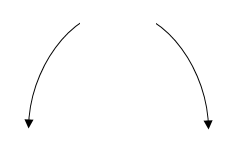
\includegraphics[width = 0.3\textwidth]{../Figures/polyEndBehaviorBA.png}
\item 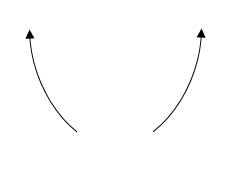
\includegraphics[width = 0.3\textwidth]{../Figures/polyEndBehaviorCA.png}
\item 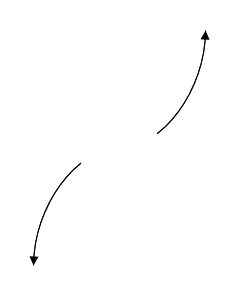
\includegraphics[width = 0.3\textwidth]{../Figures/polyEndBehaviorDA.png}
\end{multicols}\item None of the above.\end{enumerate}
\textbf{General Comment:} Remember that end behavior is determined by the leading coefficient AND whether the \textbf{sum} of the multiplicities is positive or negative.
}
\litem{
Construct the lowest-degree polynomial given the zeros below. Then, choose the intervals that contain the coefficients of the polynomial in the form $ax^3+bx^2+cx+d$.
\[ \frac{-3}{2}, \frac{-4}{3}, \text{ and } \frac{-1}{4} \]The solution is \( 24x^{3} +74 x^{2} +65 x + 12 \), which is option B.\begin{enumerate}[label=\Alph*.]
\item \( a \in [21, 26], b \in [2, 9], c \in [-61, -45], \text{ and } d \in [-12, -9] \)

$24x^{3} +2 x^{2} -49 x -12$, which corresponds to multiplying out $(2x -3)(3x + 4)(4x + 1)$.
\item \( a \in [21, 26], b \in [69, 75], c \in [60, 68], \text{ and } d \in [9, 16] \)

* $24x^{3} +74 x^{2} +65 x + 12$, which is the correct option.
\item \( a \in [21, 26], b \in [-68, -61], c \in [27, 37], \text{ and } d \in [9, 16] \)

$24x^{3} -62 x^{2} +31 x + 12$, which corresponds to multiplying out $(2x -3)(3x -4)(4x + 1)$.
\item \( a \in [21, 26], b \in [69, 75], c \in [60, 68], \text{ and } d \in [-12, -9] \)

$24x^{3} +74 x^{2} +65 x -12$, which corresponds to multiplying everything correctly except the constant term.
\item \( a \in [21, 26], b \in [-77, -65], c \in [60, 68], \text{ and } d \in [-12, -9] \)

$24x^{3} -74 x^{2} +65 x -12$, which corresponds to multiplying out $(2x -3)(3x -4)(4x -1)$.
\end{enumerate}

\textbf{General Comment:} To construct the lowest-degree polynomial, you want to multiply out $(2x + 3)(3x + 4)(4x + 1)$
}
\litem{
Construct the lowest-degree polynomial given the zeros below. Then, choose the intervals that contain the coefficients of the polynomial in the form $ax^3+bx^2+cx+d$.
\[ \frac{-5}{3}, \frac{3}{5}, \text{ and } \frac{-4}{3} \]The solution is \( 45x^{3} +108 x^{2} +19 x -60 \), which is option A.\begin{enumerate}[label=\Alph*.]
\item \( a \in [42, 46], b \in [107, 114], c \in [12, 24], \text{ and } d \in [-67, -56] \)

* $45x^{3} +108 x^{2} +19 x -60$, which is the correct option.
\item \( a \in [42, 46], b \in [-42, -40], c \in [-92, -85], \text{ and } d \in [59, 61] \)

$45x^{3} -42 x^{2} -91 x + 60$, which corresponds to multiplying out $(3x -5)(5x -3)(3x + 4)$.
\item \( a \in [42, 46], b \in [9, 14], c \in [-111, -107], \text{ and } d \in [-67, -56] \)

$45x^{3} +12 x^{2} -109 x -60$, which corresponds to multiplying out $(3x -5)(5x + 3)(3x + 4)$.
\item \( a \in [42, 46], b \in [-114, -106], c \in [12, 24], \text{ and } d \in [59, 61] \)

$45x^{3} -108 x^{2} +19 x + 60$, which corresponds to multiplying out $(3x -5)(5x + 3)(3x -4)$.
\item \( a \in [42, 46], b \in [107, 114], c \in [12, 24], \text{ and } d \in [59, 61] \)

$45x^{3} +108 x^{2} +19 x + 60$, which corresponds to multiplying everything correctly except the constant term.
\end{enumerate}

\textbf{General Comment:} To construct the lowest-degree polynomial, you want to multiply out $(3x + 5)(5x -3)(3x + 4)$
}
\litem{
Describe the zero behavior of the zero $x = 6$ of the polynomial below.
\[ f(x) = -3(x + 5)^{10}(x - 5)^{7}(x - 6)^{12}(x + 6)^{9} \]The solution is the graph below, which is option B.
    \begin{center}
        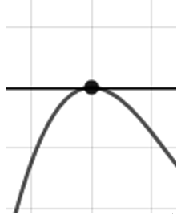
\includegraphics[width=0.3\textwidth]{../Figures/polyZeroBehaviorBB.png}
    \end{center}\begin{enumerate}[label=\Alph*.]
\begin{multicols}{2}
\item 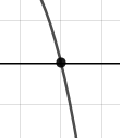
\includegraphics[width = 0.3\textwidth]{../Figures/polyZeroBehaviorAB.png}
\item 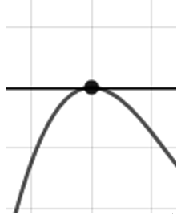
\includegraphics[width = 0.3\textwidth]{../Figures/polyZeroBehaviorBB.png}
\item 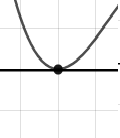
\includegraphics[width = 0.3\textwidth]{../Figures/polyZeroBehaviorCB.png}
\item 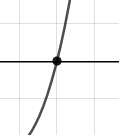
\includegraphics[width = 0.3\textwidth]{../Figures/polyZeroBehaviorDB.png}
\end{multicols}\item None of the above.\end{enumerate}
\textbf{General Comment:} You will need to sketch the entire graph, then zoom in on the zero the question asks about.
}
\litem{
Construct the lowest-degree polynomial given the zeros below. Then, choose the intervals that contain the coefficients of the polynomial in the form $x^3+bx^2+cx+d$.
\[ 4 - 5 i \text{ and } -2 \]The solution is \( x^{3} -6 x^{2} +25 x + 82 \), which is option D.\begin{enumerate}[label=\Alph*.]
\item \( b \in [1, 2], c \in [6, 8], \text{ and } d \in [9, 16] \)

$x^{3} + x^{2} +7 x + 10$, which corresponds to multiplying out $(x + 5)(x + 2)$.
\item \( b \in [6, 8], c \in [22, 31], \text{ and } d \in [-87, -77] \)

$x^{3} +6 x^{2} +25 x -82$, which corresponds to multiplying out $(x-(4 - 5 i))(x-(4 + 5 i))(x -2)$.
\item \( b \in [1, 2], c \in [-8, 5], \text{ and } d \in [-12, -6] \)

$x^{3} + x^{2} -2 x -8$, which corresponds to multiplying out $(x -4)(x + 2)$.
\item \( b \in [-6, -2], c \in [22, 31], \text{ and } d \in [75, 87] \)

* $x^{3} -6 x^{2} +25 x + 82$, which is the correct option.
\item \( \text{None of the above.} \)

This corresponds to making an unanticipated error or not understanding how to use nonreal complex numbers to create the lowest-degree polynomial. If you chose this and are not sure what you did wrong, please contact the coordinator for help.
\end{enumerate}

\textbf{General Comment:} Remember that the conjugate of $a+bi$ is $a-bi$. Since these zeros always come in pairs, we need to multiply out $(x-(4 - 5 i))(x-(4 + 5 i))(x-(-2))$.
}
\litem{
Which of the following equations \textit{could} be of the graph presented below?

\begin{center}
    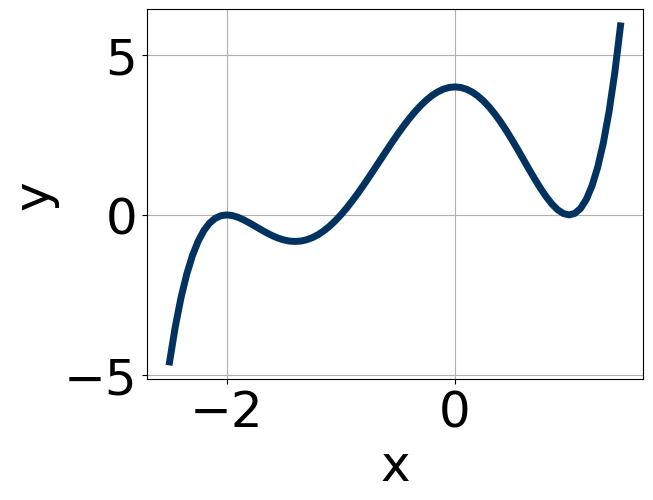
\includegraphics[width=0.5\textwidth]{../Figures/polyGraphToFunctionCopyB.png}
\end{center}


The solution is \( 10(x + 2)^{6} (x - 1)^{6} (x + 1)^{5} \), which is option B.\begin{enumerate}[label=\Alph*.]
\item \( -8(x + 2)^{10} (x - 1)^{6} (x + 1)^{8} \)

The factor $(x + 1)$ should have an odd power and the leading coefficient should be the opposite sign.
\item \( 10(x + 2)^{6} (x - 1)^{6} (x + 1)^{5} \)

* This is the correct option.
\item \( -15(x + 2)^{6} (x - 1)^{4} (x + 1)^{9} \)

This corresponds to the leading coefficient being the opposite value than it should be.
\item \( 5(x + 2)^{10} (x - 1)^{11} (x + 1)^{7} \)

The factor $(x - 1)$ should have an even power.
\item \( 15(x + 2)^{10} (x - 1)^{9} (x + 1)^{6} \)

The factor $(x - 1)$ should have an even power and the factor $(x + 1)$ should have an odd power.
\end{enumerate}

\textbf{General Comment:} General Comments: Draw the x-axis to determine which zeros are touching (and so have even multiplicity) or cross (and have odd multiplicity).
}
\litem{
Describe the zero behavior of the zero $x = -6$ of the polynomial below.
\[ f(x) = -9(x - 6)^{9}(x + 6)^{14}(x + 3)^{4}(x - 3)^{6} \]The solution is the graph below, which is option C.
    \begin{center}
        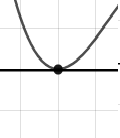
\includegraphics[width=0.3\textwidth]{../Figures/polyZeroBehaviorCopyCB.png}
    \end{center}\begin{enumerate}[label=\Alph*.]
\begin{multicols}{2}
\item 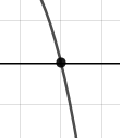
\includegraphics[width = 0.3\textwidth]{../Figures/polyZeroBehaviorCopyAB.png}
\item 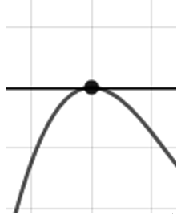
\includegraphics[width = 0.3\textwidth]{../Figures/polyZeroBehaviorCopyBB.png}
\item 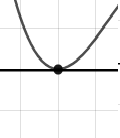
\includegraphics[width = 0.3\textwidth]{../Figures/polyZeroBehaviorCopyCB.png}
\item 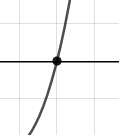
\includegraphics[width = 0.3\textwidth]{../Figures/polyZeroBehaviorCopyDB.png}
\end{multicols}\item None of the above.\end{enumerate}
\textbf{General Comment:} You will need to sketch the entire graph, then zoom in on the zero the question asks about.
}
\litem{
Which of the following equations \textit{could} be of the graph presented below?

\begin{center}
    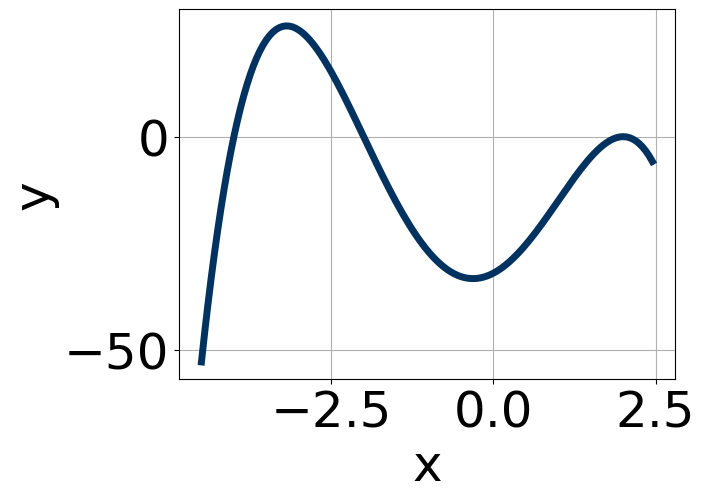
\includegraphics[width=0.5\textwidth]{../Figures/polyGraphToFunctionB.png}
\end{center}


The solution is \( -11(x - 2)^{6} (x + 2)^{11} (x + 4)^{7} \), which is option E.\begin{enumerate}[label=\Alph*.]
\item \( 13(x - 2)^{8} (x + 2)^{11} (x + 4)^{10} \)

The factor $(x + 4)$ should have an odd power and the leading coefficient should be the opposite sign.
\item \( 4(x - 2)^{6} (x + 2)^{5} (x + 4)^{9} \)

This corresponds to the leading coefficient being the opposite value than it should be.
\item \( -12(x - 2)^{10} (x + 2)^{8} (x + 4)^{7} \)

The factor $(x + 2)$ should have an odd power.
\item \( -14(x - 2)^{7} (x + 2)^{4} (x + 4)^{9} \)

The factor $2$ should have an even power and the factor $-2$ should have an odd power.
\item \( -11(x - 2)^{6} (x + 2)^{11} (x + 4)^{7} \)

* This is the correct option.
\end{enumerate}

\textbf{General Comment:} General Comments: Draw the x-axis to determine which zeros are touching (and so have even multiplicity) or cross (and have odd multiplicity).
}
\litem{
Construct the lowest-degree polynomial given the zeros below. Then, choose the intervals that contain the coefficients of the polynomial in the form $x^3+bx^2+cx+d$.
\[ -5 + 4 i \text{ and } -3 \]The solution is \( x^{3} +13 x^{2} +71 x + 123 \), which is option D.\begin{enumerate}[label=\Alph*.]
\item \( b \in [-7, 6], c \in [1, 11], \text{ and } d \in [8, 23] \)

$x^{3} + x^{2} +8 x + 15$, which corresponds to multiplying out $(x + 5)(x + 3)$.
\item \( b \in [-7, 6], c \in [-6, 2], \text{ and } d \in [-15, -11] \)

$x^{3} + x^{2} -x -12$, which corresponds to multiplying out $(x -4)(x + 3)$.
\item \( b \in [-22, -12], c \in [69, 77], \text{ and } d \in [-125, -114] \)

$x^{3} -13 x^{2} +71 x -123$, which corresponds to multiplying out $(x-(-5 + 4 i))(x-(-5 - 4 i))(x -3)$.
\item \( b \in [10, 21], c \in [69, 77], \text{ and } d \in [115, 125] \)

* $x^{3} +13 x^{2} +71 x + 123$, which is the correct option.
\item \( \text{None of the above.} \)

This corresponds to making an unanticipated error or not understanding how to use nonreal complex numbers to create the lowest-degree polynomial. If you chose this and are not sure what you did wrong, please contact the coordinator for help.
\end{enumerate}

\textbf{General Comment:} Remember that the conjugate of $a+bi$ is $a-bi$. Since these zeros always come in pairs, we need to multiply out $(x-(-5 + 4 i))(x-(-5 - 4 i))(x-(-3))$.
}
\litem{
Describe the end behavior of the polynomial below.
\[ f(x) = 2(x + 9)^{3}(x - 9)^{8}(x + 5)^{3}(x - 5)^{4} \]The solution is the graph below, which is option C.
    \begin{center}
        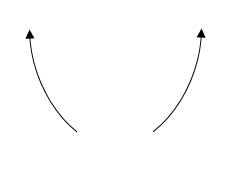
\includegraphics[width=0.3\textwidth]{../Figures/polyEndBehaviorCopyCB.png}
    \end{center}\begin{enumerate}[label=\Alph*.]
\begin{multicols}{2}
\item 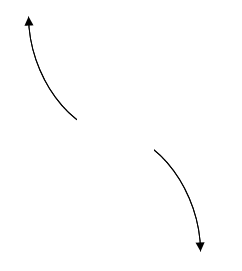
\includegraphics[width = 0.3\textwidth]{../Figures/polyEndBehaviorCopyAB.png}
\item 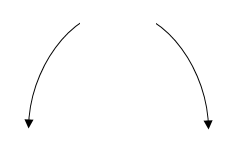
\includegraphics[width = 0.3\textwidth]{../Figures/polyEndBehaviorCopyBB.png}
\item 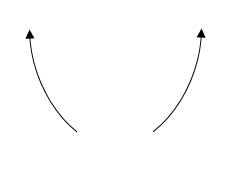
\includegraphics[width = 0.3\textwidth]{../Figures/polyEndBehaviorCopyCB.png}
\item 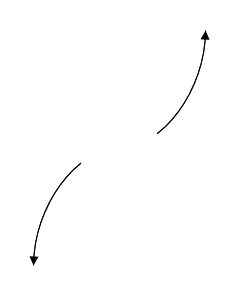
\includegraphics[width = 0.3\textwidth]{../Figures/polyEndBehaviorCopyDB.png}
\end{multicols}\item None of the above.\end{enumerate}
\textbf{General Comment:} Remember that end behavior is determined by the leading coefficient AND whether the \textbf{sum} of the multiplicities is positive or negative.
}
\litem{
Describe the end behavior of the polynomial below.
\[ f(x) = -7(x - 4)^{5}(x + 4)^{6}(x - 5)^{4}(x + 5)^{6} \]The solution is the graph below, which is option A.
    \begin{center}
        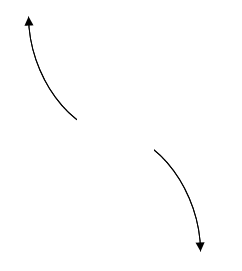
\includegraphics[width=0.3\textwidth]{../Figures/polyEndBehaviorAB.png}
    \end{center}\begin{enumerate}[label=\Alph*.]
\begin{multicols}{2}
\item 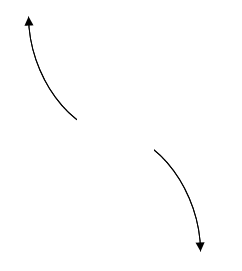
\includegraphics[width = 0.3\textwidth]{../Figures/polyEndBehaviorAB.png}
\item 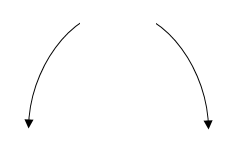
\includegraphics[width = 0.3\textwidth]{../Figures/polyEndBehaviorBB.png}
\item 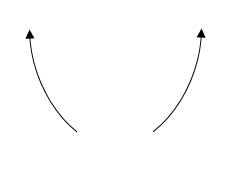
\includegraphics[width = 0.3\textwidth]{../Figures/polyEndBehaviorCB.png}
\item 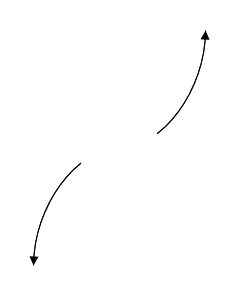
\includegraphics[width = 0.3\textwidth]{../Figures/polyEndBehaviorDB.png}
\end{multicols}\item None of the above.\end{enumerate}
\textbf{General Comment:} Remember that end behavior is determined by the leading coefficient AND whether the \textbf{sum} of the multiplicities is positive or negative.
}
\litem{
Construct the lowest-degree polynomial given the zeros below. Then, choose the intervals that contain the coefficients of the polynomial in the form $ax^3+bx^2+cx+d$.
\[ \frac{-1}{3}, 1, \text{ and } \frac{-2}{5} \]The solution is \( 15x^{3} -4 x^{2} -9 x -2 \), which is option C.\begin{enumerate}[label=\Alph*.]
\item \( a \in [10, 17], b \in [3, 11], c \in [-9.39, -8.23], \text{ and } d \in [-0.3, 4.6] \)

$15x^{3} +4 x^{2} -9 x + 2$, which corresponds to multiplying out $(3x -1)(x + 1)(5x -2)$.
\item \( a \in [10, 17], b \in [10, 23], c \in [-1.88, -0.96], \text{ and } d \in [-2.8, -0.2] \)

$15x^{3} +16 x^{2} -x -2$, which corresponds to multiplying out $(3x -1)(x + 1)(5x + 2)$.
\item \( a \in [10, 17], b \in [-7, -3], c \in [-9.39, -8.23], \text{ and } d \in [-2.8, -0.2] \)

* $15x^{3} -4 x^{2} -9 x -2$, which is the correct option.
\item \( a \in [10, 17], b \in [-7, -3], c \in [-9.39, -8.23], \text{ and } d \in [-0.3, 4.6] \)

$15x^{3} -4 x^{2} -9 x + 2$, which corresponds to multiplying everything correctly except the constant term.
\item \( a \in [10, 17], b \in [-18, -11], c \in [-4.09, -2.6], \text{ and } d \in [-0.3, 4.6] \)

$15x^{3} -14 x^{2} -3 x + 2$, which corresponds to multiplying out $(3x -1)(x -1)(5x + 2)$.
\end{enumerate}

\textbf{General Comment:} To construct the lowest-degree polynomial, you want to multiply out $(3x + 1)(x -1)(5x + 2)$
}
\litem{
Construct the lowest-degree polynomial given the zeros below. Then, choose the intervals that contain the coefficients of the polynomial in the form $ax^3+bx^2+cx+d$.
\[ \frac{7}{3}, 1, \text{ and } \frac{-7}{2} \]The solution is \( 6x^{3} + x^{2} -56 x + 49 \), which is option C.\begin{enumerate}[label=\Alph*.]
\item \( a \in [0, 14], b \in [28, 31.1], c \in [12, 15], \text{ and } d \in [-57, -44] \)

$6x^{3} +29 x^{2} +14 x -49$, which corresponds to multiplying out $(3x + 7)(x -1)(2x + 7)$.
\item \( a \in [0, 14], b \in [0.9, 2], c \in [-60, -55], \text{ and } d \in [-57, -44] \)

$6x^{3} + x^{2} -56 x -49$, which corresponds to multiplying everything correctly except the constant term.
\item \( a \in [0, 14], b \in [0.9, 2], c \in [-60, -55], \text{ and } d \in [48, 54] \)

* $6x^{3} + x^{2} -56 x + 49$, which is the correct option.
\item \( a \in [0, 14], b \in [40.6, 41.8], c \in [82, 89], \text{ and } d \in [48, 54] \)

$6x^{3} +41 x^{2} +84 x + 49$, which corresponds to multiplying out $(3x + 7)(x + 1)(2x + 7)$.
\item \( a \in [0, 14], b \in [-4.2, 0.2], c \in [-60, -55], \text{ and } d \in [-57, -44] \)

$6x^{3} -1 x^{2} -56 x -49$, which corresponds to multiplying out $(3x + 7)(x + 1)(2x -7)$.
\end{enumerate}

\textbf{General Comment:} To construct the lowest-degree polynomial, you want to multiply out $(3x -7)(x -1)(2x + 7)$
}
\litem{
Describe the zero behavior of the zero $x = -4$ of the polynomial below.
\[ f(x) = -4(x + 4)^{5}(x - 4)^{8}(x - 9)^{3}(x + 9)^{4} \]The solution is the graph below, which is option D.
    \begin{center}
        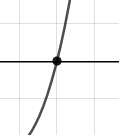
\includegraphics[width=0.3\textwidth]{../Figures/polyZeroBehaviorDC.png}
    \end{center}\begin{enumerate}[label=\Alph*.]
\begin{multicols}{2}
\item 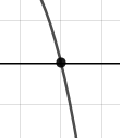
\includegraphics[width = 0.3\textwidth]{../Figures/polyZeroBehaviorAC.png}
\item 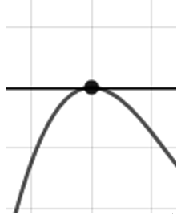
\includegraphics[width = 0.3\textwidth]{../Figures/polyZeroBehaviorBC.png}
\item 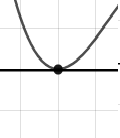
\includegraphics[width = 0.3\textwidth]{../Figures/polyZeroBehaviorCC.png}
\item 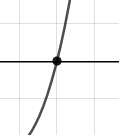
\includegraphics[width = 0.3\textwidth]{../Figures/polyZeroBehaviorDC.png}
\end{multicols}\item None of the above.\end{enumerate}
\textbf{General Comment:} You will need to sketch the entire graph, then zoom in on the zero the question asks about.
}
\litem{
Construct the lowest-degree polynomial given the zeros below. Then, choose the intervals that contain the coefficients of the polynomial in the form $x^3+bx^2+cx+d$.
\[ 5 - 2 i \text{ and } 1 \]The solution is \( x^{3} -11 x^{2} +39 x -29 \), which is option A.\begin{enumerate}[label=\Alph*.]
\item \( b \in [-14, -9], c \in [37, 44], \text{ and } d \in [-34, -23] \)

* $x^{3} -11 x^{2} +39 x -29$, which is the correct option.
\item \( b \in [2, 13], c \in [37, 44], \text{ and } d \in [27, 33] \)

$x^{3} +11 x^{2} +39 x + 29$, which corresponds to multiplying out $(x-(5 - 2 i))(x-(5 + 2 i))(x + 1)$.
\item \( b \in [-2, 6], c \in [-2, 5], \text{ and } d \in [-6, 1] \)

$x^{3} + x^{2} +x -2$, which corresponds to multiplying out $(x + 2)(x -1)$.
\item \( b \in [-2, 6], c \in [-6, -5], \text{ and } d \in [0, 8] \)

$x^{3} + x^{2} -6 x + 5$, which corresponds to multiplying out $(x -5)(x -1)$.
\item \( \text{None of the above.} \)

This corresponds to making an unanticipated error or not understanding how to use nonreal complex numbers to create the lowest-degree polynomial. If you chose this and are not sure what you did wrong, please contact the coordinator for help.
\end{enumerate}

\textbf{General Comment:} Remember that the conjugate of $a+bi$ is $a-bi$. Since these zeros always come in pairs, we need to multiply out $(x-(5 - 2 i))(x-(5 + 2 i))(x-(1))$.
}
\litem{
Which of the following equations \textit{could} be of the graph presented below?

\begin{center}
    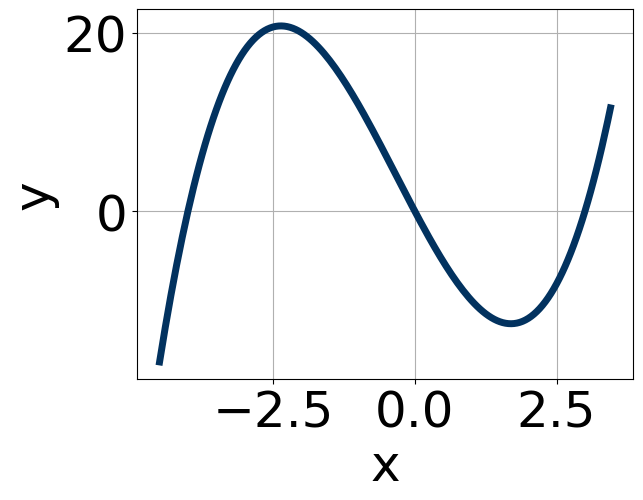
\includegraphics[width=0.5\textwidth]{../Figures/polyGraphToFunctionCopyC.png}
\end{center}


The solution is \( 7x^{9} (x + 4)^{11} (x - 3)^{9} \), which is option B.\begin{enumerate}[label=\Alph*.]
\item \( -11x^{6} (x + 4)^{11} (x - 3)^{5} \)

The factor $x$ should have an odd power and the leading coefficient should be the opposite sign.
\item \( 7x^{9} (x + 4)^{11} (x - 3)^{9} \)

* This is the correct option.
\item \( -6x^{7} (x + 4)^{5} (x - 3)^{5} \)

This corresponds to the leading coefficient being the opposite value than it should be.
\item \( 6x^{8} (x + 4)^{4} (x - 3)^{11} \)

The factors $0$ and $-4$ have have been odd power.
\item \( 8x^{8} (x + 4)^{5} (x - 3)^{7} \)

The factor $0$ should have been an odd power.
\end{enumerate}

\textbf{General Comment:} General Comments: Draw the x-axis to determine which zeros are touching (and so have even multiplicity) or cross (and have odd multiplicity).
}
\litem{
Describe the zero behavior of the zero $x = -8$ of the polynomial below.
\[ f(x) = 4(x - 7)^{5}(x + 7)^{3}(x + 8)^{9}(x - 8)^{8} \]The solution is the graph below, which is option D.
    \begin{center}
        \includegraphics[width=0.3\textwidth]{../Figures/polyZeroBehaviorCopyDC.png}
    \end{center}\begin{enumerate}[label=\Alph*.]
\begin{multicols}{2}
\item \includegraphics[width = 0.3\textwidth]{../Figures/polyZeroBehaviorCopyAC.png}
\item \includegraphics[width = 0.3\textwidth]{../Figures/polyZeroBehaviorCopyBC.png}
\item \includegraphics[width = 0.3\textwidth]{../Figures/polyZeroBehaviorCopyCC.png}
\item \includegraphics[width = 0.3\textwidth]{../Figures/polyZeroBehaviorCopyDC.png}
\end{multicols}\item None of the above.\end{enumerate}
\textbf{General Comment:} You will need to sketch the entire graph, then zoom in on the zero the question asks about.
}
\litem{
Which of the following equations \textit{could} be of the graph presented below?

\begin{center}
    \includegraphics[width=0.5\textwidth]{../Figures/polyGraphToFunctionC.png}
\end{center}


The solution is \( -4(x + 4)^{4} (x - 3)^{10} (x + 3)^{4} \), which is option B.\begin{enumerate}[label=\Alph*.]
\item \( 16(x + 4)^{10} (x - 3)^{10} (x + 3)^{6} \)

This corresponds to the leading coefficient being the opposite value than it should be.
\item \( -4(x + 4)^{4} (x - 3)^{10} (x + 3)^{4} \)

* This is the correct option.
\item \( 14(x + 4)^{10} (x - 3)^{4} (x + 3)^{11} \)

The factor $(x + 3)$ should have an even power and the leading coefficient should be the opposite sign.
\item \( -7(x + 4)^{4} (x - 3)^{11} (x + 3)^{7} \)

The factors $(x - 3)$ and $(x + 3)$ should both have even powers.
\item \( -10(x + 4)^{10} (x - 3)^{6} (x + 3)^{11} \)

The factor $(x + 3)$ should have an even power.
\end{enumerate}

\textbf{General Comment:} General Comments: Draw the x-axis to determine which zeros are touching (and so have even multiplicity) or cross (and have odd multiplicity).
}
\litem{
Construct the lowest-degree polynomial given the zeros below. Then, choose the intervals that contain the coefficients of the polynomial in the form $x^3+bx^2+cx+d$.
\[ 5 - 2 i \text{ and } 4 \]The solution is \( x^{3} -14 x^{2} +69 x -116 \), which is option A.\begin{enumerate}[label=\Alph*.]
\item \( b \in [-17, -13], c \in [69, 79], \text{ and } d \in [-116, -115] \)

* $x^{3} -14 x^{2} +69 x -116$, which is the correct option.
\item \( b \in [-7, 5], c \in [-5, 6], \text{ and } d \in [-9, -2] \)

$x^{3} + x^{2} -2 x -8$, which corresponds to multiplying out $(x + 2)(x -4)$.
\item \( b \in [-7, 5], c \in [-13, -6], \text{ and } d \in [10, 27] \)

$x^{3} + x^{2} -9 x + 20$, which corresponds to multiplying out $(x -5)(x -4)$.
\item \( b \in [14, 16], c \in [69, 79], \text{ and } d \in [114, 119] \)

$x^{3} +14 x^{2} +69 x + 116$, which corresponds to multiplying out $(x-(5 - 2 i))(x-(5 + 2 i))(x + 4)$.
\item \( \text{None of the above.} \)

This corresponds to making an unanticipated error or not understanding how to use nonreal complex numbers to create the lowest-degree polynomial. If you chose this and are not sure what you did wrong, please contact the coordinator for help.
\end{enumerate}

\textbf{General Comment:} Remember that the conjugate of $a+bi$ is $a-bi$. Since these zeros always come in pairs, we need to multiply out $(x-(5 - 2 i))(x-(5 + 2 i))(x-(4))$.
}
\litem{
Describe the end behavior of the polynomial below.
\[ f(x) = -9(x + 2)^{4}(x - 2)^{5}(x - 6)^{5}(x + 6)^{7} \]The solution is the graph below, which is option A.
    \begin{center}
        \includegraphics[width=0.3\textwidth]{../Figures/polyEndBehaviorCopyAC.png}
    \end{center}\begin{enumerate}[label=\Alph*.]
\begin{multicols}{2}
\item \includegraphics[width = 0.3\textwidth]{../Figures/polyEndBehaviorCopyAC.png}
\item \includegraphics[width = 0.3\textwidth]{../Figures/polyEndBehaviorCopyBC.png}
\item \includegraphics[width = 0.3\textwidth]{../Figures/polyEndBehaviorCopyCC.png}
\item \includegraphics[width = 0.3\textwidth]{../Figures/polyEndBehaviorCopyDC.png}
\end{multicols}\item None of the above.\end{enumerate}
\textbf{General Comment:} Remember that end behavior is determined by the leading coefficient AND whether the \textbf{sum} of the multiplicities is positive or negative.
}
\litem{
Describe the end behavior of the polynomial below.
\[ f(x) = 9(x + 3)^{2}(x - 3)^{3}(x - 4)^{4}(x + 4)^{5} \]The solution is the graph below, which is option C.
    \begin{center}
        \includegraphics[width=0.3\textwidth]{../Figures/polyEndBehaviorCC.png}
    \end{center}\begin{enumerate}[label=\Alph*.]
\begin{multicols}{2}
\item \includegraphics[width = 0.3\textwidth]{../Figures/polyEndBehaviorAC.png}
\item \includegraphics[width = 0.3\textwidth]{../Figures/polyEndBehaviorBC.png}
\item \includegraphics[width = 0.3\textwidth]{../Figures/polyEndBehaviorCC.png}
\item \includegraphics[width = 0.3\textwidth]{../Figures/polyEndBehaviorDC.png}
\end{multicols}\item None of the above.\end{enumerate}
\textbf{General Comment:} Remember that end behavior is determined by the leading coefficient AND whether the \textbf{sum} of the multiplicities is positive or negative.
}
\litem{
Construct the lowest-degree polynomial given the zeros below. Then, choose the intervals that contain the coefficients of the polynomial in the form $ax^3+bx^2+cx+d$.
\[ \frac{-7}{4}, \frac{-7}{5}, \text{ and } 4 \]The solution is \( 20x^{3} -17 x^{2} -203 x -196 \), which is option C.\begin{enumerate}[label=\Alph*.]
\item \( a \in [20, 23], b \in [-144, -139], c \in [301, 307], \text{ and } d \in [-196, -195] \)

$20x^{3} -143 x^{2} +301 x -196$, which corresponds to multiplying out $(4x -7)(5x -7)(x -4)$.
\item \( a \in [20, 23], b \in [9, 18], c \in [-207, -199], \text{ and } d \in [189, 200] \)

$20x^{3} +17 x^{2} -203 x + 196$, which corresponds to multiplying out $(4x -7)(5x -7)(x + 4)$.
\item \( a \in [20, 23], b \in [-19, -15], c \in [-207, -199], \text{ and } d \in [-196, -195] \)

* $20x^{3} -17 x^{2} -203 x -196$, which is the correct option.
\item \( a \in [20, 23], b \in [-92, -78], c \in [-26, -20], \text{ and } d \in [189, 200] \)

$20x^{3} -87 x^{2} -21 x + 196$, which corresponds to multiplying out $(4x -7)(5x + 7)(x -4)$.
\item \( a \in [20, 23], b \in [-19, -15], c \in [-207, -199], \text{ and } d \in [189, 200] \)

$20x^{3} -17 x^{2} -203 x + 196$, which corresponds to multiplying everything correctly except the constant term.
\end{enumerate}

\textbf{General Comment:} To construct the lowest-degree polynomial, you want to multiply out $(4x + 7)(5x + 7)(x -4)$
}
\end{enumerate}

\end{document}